% CVPR 2025 Paper Template; see https://github.com/cvpr-org/author-kit
\documentclass[10pt,twocolumn,letterpaper]{article}

%%%%%%%%% PAPER TYPE  - PLEASE UPDATE FOR FINAL VERSION
% \usepackage{cvpr}              % To produce the CAMERA-READY version
\usepackage[review]{cvpr}      % To produce the REVIEW version
% \usepackage[pagenumbers]{cvpr} % To force page numbers, e.g. for an arXiv version

% Import additional packages in the preamble file, before hyperref
\input{cvpr_kit_min/preamble}

% Additional packages used by this paper (before hyperref)
\usepackage{tikz}
\usetikzlibrary{arrows.meta,positioning,fit,calc,shapes.misc}
\usepackage{pgfplots}
\pgfplotsset{compat=1.18}
\usepackage[ruled,vlined]{algorithm2e}
\usepackage{float}
\usepackage{adjustbox}
\usepackage{multirow}
% For including SVGs via \includesvg
\usepackage{svg}

% It is strongly recommended to use hyperref, especially for the review version.
% hyperref with option pagebackref eases the reviewers' job.
\definecolor{cvprblue}{rgb}{0.21,0.49,0.74}
\usepackage[pagebackref,breaklinks,colorlinks,allcolors=cvprblue]{hyperref}

\input{macros}
% Centralized paper metadata shared across main/CVPR builds.
\newcommand{\papertitle}{XtoCIF: Test-Time Scaling LLM for X-ray Diffraction}

% Toggle to reveal camera-ready authors/affiliations.
\newif\ifanonymized
\anonymizedtrue

% Authblk-friendly author/affiliation block for the arXiv-style build.
\newcommand{\paperauthorblock}{%
  \author[1,2]{Germain Poloudenny}
  \author[2,3,4]{Arnaud Demortière}
  \author[1]{Ya\"el Frégier}
  \affil[1]{Laboratoire de Mathématiques de Lens (LML), Université d'Artois, Lens, France}
  \affil[2]{Laboratoire de Réactivité et de Chimie des Solides, CNRS UMR 7314, Université de Picardie Jules Verne, Hub de l’Energie, Rue Baudelocque, Amiens, France}
  \affil[3]{Réseau sur le Stockage Electrochimique de l’Energie (RS2E), CNRS FR 3459, Hub de l’Energie, Rue Baudelocque, Amiens, France}
  \affil[4]{ALISTORE-European Research Institute, CNRS FR 3104, Hub de l’Energie, Rue Baudelocque, Amiens, France}
}

% Compact strings for templates that require single \author blocks (e.g., CVPR).
\newcommand{\paperauthorline}{Germain Poloudenny$^{1,2}$, Arnaud Demortière$^{2,3,4}$, Ya\"el Frégier$^{1}$}
\newcommand{\paperaffilline}{%
  $^{1}$LML, Université d'Artois, Lens, France\\%
  $^{2}$LRCS, CNRS UMR 7314, UPJV, Amiens, France\\%
  $^{3}$RS2E, CNRS FR 3459, Amiens, France\\%
  $^{4}$ALISTORE-ERI, CNRS FR 3104, Amiens, France%
}

% CVPR submission metadata
% Replace with your assigned Paper ID from OpenReview before submission
\newcommand{\paperID}{29506}


%%%%%%%%% PAPER ID  - PLEASE UPDATE
% Paper ID is defined in paper_metadata.tex as \paperID
\def\confName{CVPR}
\def\confYear{2025}

%%%%%%%%% TITLE - PLEASE UPDATE
\title{\papertitle}

%%%%%%%%% AUTHORS - ANONYMIZED FOR REVIEW
\ifanonymized
  \author{Anonymous CVPR submission\\Paper ID \paperID}
\else
  \author{\paperauthorline\\[3pt]\paperaffilline}
\fi

\begin{document}
\maketitle

% Abstract and content
\begin{abstract}
Automated crystal structure prediction (CSP) can accelerate materials discovery by combining experimental data with generative models. \xtoCIF builds on \deCIFer and retains the original autoregressive architecture and tokenizer. We introduce engineering improvements and a standardized powder X‑ray diffraction (PXRD) evaluation protocol. The main changes are a GPU‑optimized training pipeline with approximately \(44\times\) higher throughput, deterministic beam search decoding, diffraction‑aware reranking using the weighted‑profile residual \(\Rwp\), and a unified evaluation suite that covers descriptor‑free, composition, and composition‑plus‑space‑group conditioning.

On NOMA, the descriptor‑free setting benefits most: \(\Rwp\) decreases from 0.23 to 0.18 while the structural match rate (MR) increases from 5.6~\% to 8.1~\%. With composition or composition‑plus‑space‑group conditioning, MR rises from the \deCIFer baseline of \(\approx94~\%\) to \(\approx97~\%\) while \(\Rwp\) drops further. These gains arise from training, decoding, and evaluation engineering rather than architectural changes—the generator and tokenizer are unchanged. In practice we recommend a simple default: deterministic beam search with width \(B{=}5\) followed by \(\Rwp\)‑based reranking, which consistently improves over greedy sampling at modest compute cost.
\end{abstract}

% Cleaned template body generated from content.tex
% - Keeps section hierarchy and labels
% - Removes paragraphs, figures, tables, equations, citations, etc.
% - Replace TODO stubs with your text

\section{Introduction}

Powder X-ray diffraction (PXRD) is the most widely available probe for characterizing crystalline intermediates, yet turning a noisy one-dimensional scattering profile into an atomic structure still hinges on manual Rietveld-style refinement, curated priors, and hours of expert iteration~\cite{toby2013gsas2,rodriguezcarvajal1993fullprof,Cheetham2014}. Fully autonomous PXRD workflows therefore require models that can translate raw intensities into crystallographic information files (CIFs) while remaining faithful to experimental noise and instrument effects.

Autoregressive language models conditioned on PXRD embeddings (\eg, \deCIFer~\cite{deCIFer2025}) have taken important steps in this direction by directly generating CIF tokens from diffraction traces. However, the baseline exposed three systemic bottlenecks: (i) multi-day training due to inefficient data serving and augmentation, (ii) a single decoding rule that selects candidates solely by language-model likelihood, without a separate PXRD-based scoring step, and (iii) ad hoc evaluation of candidate CIF portfolios when chemical composition or symmetry descriptors are missing.

We introduce \xtoCIF, a practitioner-oriented extension that revisits training, decoding, and evaluation for PXRD-to-structure models. The framework accelerates data loading and PXRD augmentation, exposes scriptable deterministic beam search alongside the default stochastic sampler, and provides utilities that order candidate CIFs by their post hoc weighted-profile residual (\(\Rwp\)). Collectively, these changes enable systematic comparison across descriptor‑free, composition-conditioned, and composition‑plus‑space‑group regimes without altering the underlying autoregressive architecture or tokenizer.

On the NOMA benchmark, the proposed training stack delivers \(\sim44\times\) higher throughput while maintaining fidelity to experimental artifacts, and the decoding protocol improves both match rate (MR) and \(\Rwp\) in low-information settings. For comparability, we retain the MR, validity, and \(\Rwp\) metrics established by \deCIFer and report all ablations in the same evaluation harness.


\paragraph{Contributions.} Relative to \deCIFer, \xtoCIF keeps the autoregressive generator and tokenizer unchanged. We contribute three self-contained, quantified components:
\begin{itemize}
  \item \textbf{Training system (engineering).} A GPU-optimized pipeline that delivers \(\sim\!44\times\) higher throughput on NOMA via streamlined data serving, efficient PXRD augmentation, and multi-GPU orchestration. Single-GPU iteration time drops from \(257.9\!\pm\!4.2\) s to \(10.35\!\pm\!0.13\) s, and to \(5.82\!\pm\!0.19\) s on 2 GPUs (\(124\!\pm\!2\) and \(220\!\pm\!7\) samples/s respectively), reducing wall-clock training time by roughly \(44\times\) for a fixed step budget (Table~\ref{tab:train-optimization-throughput}). This acceleration allowed us to sweep dozens of random seeds and initialization strategies, raising the composition-conditioned MR to \(\approx97\%\) without modifying the \deCIFer backbone (Table~\ref{tab:decoding_refinements}); the original \deCIFer report lists \(\approx94\%\) for this regime~\cite{deCIFer2025}.
  \item \textbf{Inference protocol.} We expose deterministic beam search alongside the stochastic sampler and make it easy to sweep beam widths through the shared evaluation harness. Candidates are subsequently ordered by their computed \(\Rwp\) using the same utilities, which enables post hoc filtering of the beam without modifying checkpoints. In the descriptor‑free regime on NOMA this workflow reduces \(\Rwp\) from 0.23 to 0.18 and raises match rate (MR) from 5.6\% to 8.1\% (\(+45\%\) relative); with Comp or Comp+SG, \xtoCIF keeps MR near 97.3\% while trimming \(\Rwp\) by \(\sim0.03\) (Tab.~\ref{tab:decoding_refinements}).
  \item \textbf{Evaluation protocol.} A unified, reproducible protocol across three conditioning regimes (\emph{No descriptors} / \emph{Comp} / \emph{Comp+SG}) with standardized metrics: \emph{Validity} (syntax/unit-cell parameters/bond sanity), \emph{MR} (RMSD \(\le 0.5\,\text{\AA}\) after symmetry-aware alignment that enforces chemical identity), and \(\Rwp\) computed on simulated PXRD. Unless stated otherwise, we report aggregated statistics over generated candidates (best-of-beam extracted via the post hoc filtering stage plus global medians/means). Fig.~\ref{fig:beam_rmsd_match} shows how these aggregates evolve with beam size.
\end{itemize}

% !TeX root = ../cvpr_main.tex
% Figure 1: XtoCIF overview (TikZ)
% Use [H] to prevent the figure from floating
% above the preceding paragraph (requires \usepackage{float} in the preamble).
\newcommand{\diffractogramIcon}{%
  % Fit within node width and crop out the bitmap title (keep axes only)
  % trim = left bottom right top
  \includegraphics[width=0.98\linewidth,clip,trim=0pt 0pt 0pt 28pt]{Figures/illustrations/xtocif_pxrd_input.png}%
}
\newcommand{\augmentIllustration}{%
  % Enlarge the augmentation example and crop outer whitespace
  \includegraphics[width=0.98\linewidth,clip,trim=6pt 6pt 6pt 10pt]{Figures/data_statistics/noisebroadness}%
}
% Encoder icon: use provided SVG artwork instead of the TikZ placeholder
% Source: Figures/illustrations/encoder_neural_network.svg
\newcommand{\encoderIcon}{%
  % Prefer pre-converted PDF for portability; fallback to SVG if needed
  \IfFileExists{Figures/illustrations/encoder_neural_network.pdf}{%
    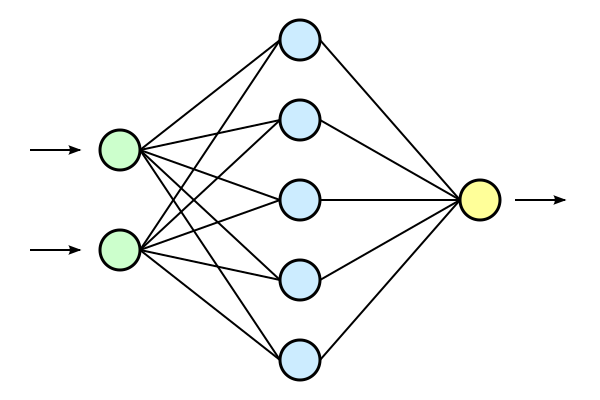
\includegraphics[width=0.98\linewidth]{Figures/illustrations/encoder_neural_network.pdf}%
  }{%
    % Requires: \usepackage{svg} in the preamble
    \includesvg[width=0.98\linewidth]{Figures/illustrations/encoder_neural_network}%
  }%
}
% --- Decoder icon: clean arrow only (sized for small block) -------------------
\newcommand{\decoderIcon}{%
  % Minimal but informative: Tokens → Decoder ×N → Logits
  \resizebox{\linewidth}{!}{%
    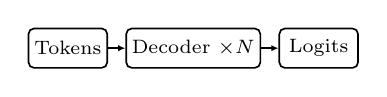
\begin{tikzpicture}[
      name prefix=decicon-,
      baseline=(current bounding box.center),
      >=Latex,
      % Ensure text inside the mini icon stays ≥7 pt
      node/.style={rounded corners=2pt, draw=black, line width=0.6pt, fill=white, minimum height=5mm, inner sep=2pt, font=\scriptsize}
    ]
      \node[node, minimum width=10mm] (tok) {Tokens};
      \node[node, minimum width=16mm, right=0.22cm of tok] (dec) {Decoder $\times N$};
      \node[node, minimum width=10mm, right=0.22cm of dec] (log) {Logits};
      \draw[-{Latex[length=2.6pt,width=2.3pt]}, line width=0.7pt] (tok.east) -- (dec.west);
      \draw[-{Latex[length=2.6pt,width=2.3pt]}, line width=0.7pt] (dec.east) -- (log.west);
    \end{tikzpicture}%
  }%
}
% Crystal structure + PXRD mini icon for simulation panel
\newcommand{\crystalPxrdIcon}{%
  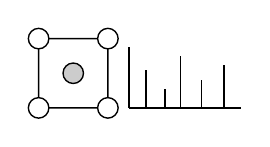
\begin{tikzpicture}[
    x=0.22cm, y=0.22cm,
    baseline=(current bounding box.center),
    atom/.style={circle, draw=black, fill=white, line width=0.5pt, inner sep=0pt, minimum size=2.6mm},
    axis/.style={line width=0.6pt}
  ]
    % Unit cell (simple square + lattice points)
    \begin{scope}[shift={(0,0)}]
      \draw[line width=0.6pt, rounded corners=1pt] (0,0) rectangle (4,4);
      \node[atom] at (0,0)    {};
      \node[atom] at (4,0)    {};
      \node[atom] at (0,4)    {};
      \node[atom] at (4,4)    {};
      \node[atom, fill=black!20] at (2,2) {};
    \end{scope}
    % Mini PXRD to the right
    \begin{scope}[shift={(5.2,0)}]
      % axes
      \draw[axis] (0,0) -- (6.5,0);
      \draw[axis] (0,0) -- (0,3.5);
      % a few peaks
      \draw[line width=0.6pt] (1.0,0) -- (1.0,2.2);
      \draw[line width=0.6pt] (2.1,0) -- (2.1,1.1);
      \draw[line width=0.6pt] (3.0,0) -- (3.0,3.0);
      \draw[line width=0.6pt] (4.2,0) -- (4.2,1.6);
      \draw[line width=0.6pt] (5.5,0) -- (5.5,2.5);
    \end{scope}
  \end{tikzpicture}%
}
% Panel for Simulate PXRD: use dataset-based image and overlay arrow (structure → PXRD)
\newcommand{\simulatePxrdPanel}{%
  % Ensure the composite panel always fits the enclosing node width
  \resizebox{\linewidth}{!}{%
    \begin{tikzpicture}[name prefix=sim-, baseline=(current bounding box.center)]
      \node[inner sep=0pt] (stru) {\includegraphics[width=0.52\linewidth]{Figures/illustrations/simulate_pxrd_ds_structure.png}};
      \node[inner sep=0pt, below=0.22cm of stru] (pxrd) {\includegraphics[width=0.74\linewidth]{Figures/illustrations/simulate_pxrd_ds_pxrd.png}};
      % Arrow starts just below structure and ends just above PXRD
      \draw[-{Latex[length=4pt,width=3.4pt]}, line width=1.0pt]
        ($(stru.south)+(0,-0.02)$) -- ($(pxrd.north)+(0,0.02)$);
    \end{tikzpicture}%
  }%
}
% Beam-search illustration sourced from the final frame of Beam\_search.gif (Wikimedia Commons)
\newcommand{\beamTreeIcon}{%
  % Crop away the black border from the source PNG
  \includegraphics[width=0.7\linewidth,clip,trim=3pt 3pt 3pt 3pt]{Figures/illustrations/beam_search_last.png}%
}
\newcommand{\rwpRankingIllustration}{%
  \includegraphics[width=0.92\linewidth]{Figures/illustrations/rwp_ranking_pxrd.png}%
}
% High-contrast fills (avoid low-contrast pastels)
\colorlet{xtoinput}{white}
\colorlet{xtomodel}{white}
\colorlet{xtodecode}{white}
\colorlet{xtoeval}{white}
% Daltonian-safe palette (Okabe–Ito)
\definecolor{oiBlue}{HTML}{0072B2}          % inherited → blue (dashed)
\definecolor{cbRed}{HTML}{E41A1C}           % contributions → true red (ColorBrewer Set1)
\colorlet{deciferOutline}{oiBlue}
\colorlet{xtocifContributionOutline}{cbRed}
\begingroup
% Tighten vertical white space around the float for CVPR columns
\setlength{\textfloatsep}{3pt plus 1pt minus 1pt}
\setlength{\intextsep}{3pt plus 1pt minus 1pt}
\begin{figure}[t]
  \centering
  % Keep within column bounds with comfortable margins under CVPR review rulers
  \begin{adjustbox}{center,max width=0.80\linewidth}
  \begin{tikzpicture}[
    >=Latex,
    % Zero outer sep so connectors touch the drawn border exactly
    % Use ≥\footnotesize everywhere for readability at 1-col scale
    block/.style={draw, rounded corners=4pt, align=center, text=black, font=\footnotesize, line width=1.0pt, inner sep=3pt, minimum height=8mm, outer sep=0pt},
    inputBlock/.style={block, fill=white},
    modelBlock/.style={block, fill=white},
    decodeBlock/.style={block, fill=white},
    evalBlock/.style={block, fill=white},
    % Connectors: main path (solid) and optional deps (dashed)
    connectorMain/.style={-{Latex[length=3pt,width=2.5pt]}, line width=0.95pt, shorten >=1.2pt, shorten <=1.2pt, line cap=round},
    connectorOpt/.style={connectorMain, dashed},
    legendBox/.style={rectangle, rounded corners=2pt, minimum width=0.5cm, minimum height=0.28cm},
    legendDot/.style={circle, minimum size=0.3cm, inner sep=0pt}
  ]
    % Unified block width
    \newlength{\xtocifBlockWidth}
    % Enlarge blocks slightly while keeping within column bounds
    \setlength{\xtocifBlockWidth}{31mm}% single source of truth
    \matrix (flow) [
      row sep=0.90cm,
      column sep=0.50cm
    ]{
      \node[inputBlock, draw=deciferOutline, dashed, text width=\xtocifBlockWidth] (pxrdIn) {\diffractogramIcon\\[1pt]\textbf{PXRD Trace $(2\theta, I)$}}; &
      \node[inputBlock, draw=deciferOutline, dashed, text width=\xtocifBlockWidth] (aug) {\textbf{Augment \& Normalize}\\[1pt]\augmentIllustration}; &
      \node[modelBlock, draw=deciferOutline, dashed, text width=\xtocifBlockWidth] (enc) {\textbf{PXRD Encoder}\\1D CNN + Transformer\\[2pt]\encoderIcon}; \\
      \node[modelBlock, draw=deciferOutline, dashed, text width=\xtocifBlockWidth] (desc) {\textbf{Descriptors $\oplus$}\\None / Comp / Comp+SG}; &
      \node[modelBlock, draw=deciferOutline, dashed, text width=\xtocifBlockWidth] (cond) {\textbf{Conditioning}}; &
      \node[modelBlock, draw=deciferOutline, dashed, text width=\xtocifBlockWidth] (decBlock) {\textbf{Decoder (AR)}\\[1pt]\decoderIcon}; \\
      \node[evalBlock, draw=xtocifContributionOutline, text width=\xtocifBlockWidth] (rwp) {\textbf{Rwp Reranking}\\[-2pt]\rwpRankingIllustration}; &
      \node[evalBlock, draw=xtocifContributionOutline, text width=\xtocifBlockWidth] (sim) {\textbf{Simulate PXRD}\\\footnotesize Per CIF\\[1pt]\simulatePxrdPanel}; &
      \node[evalBlock, draw=xtocifContributionOutline, text width=\xtocifBlockWidth] (beam) {\textbf{Beam Search}\\[1pt]\beamTreeIcon}; \\
      \node[coordinate] (gapL) {}; &
      \node[evalBlock, draw=xtocifContributionOutline, text width=\xtocifBlockWidth] (out) {\textbf{Top-k CIFs}}; &
      \node[coordinate] (gapR) {}; \\
    };

    % Flow edges (solid = main path, dashed = optional dependency)
    \draw[connectorMain] (pxrdIn) -- (aug);
    \draw[connectorMain] (aug) -- (enc);
    \draw[connectorMain] (enc) -- (cond);
    \draw[connectorOpt] (desc.east) -- (cond.west);
    % (Optional) descriptors indicated in-block via $\oplus$ symbol
    \draw[connectorMain] (cond) -- (decBlock);
    % Centered vertical link decoder → beam
    \draw[connectorMain] (decBlock.south) -- (beam.north);
    \draw[connectorMain] (beam) -- (sim);
    \draw[connectorMain] (sim) -- (rwp);
    \draw[connectorMain] (rwp.south) |- (out);

    % (Removed stage label previously reading: "PXRD observation & conditioning")

    % Compact legend: two colored pastilles (dashed = inherited, solid = contributions)
    % Compact legend placed to the right of Top-K block
    \matrix (legend) [
      font=\scriptsize,
      column sep=2mm,
      row sep=0.5mm,
      anchor=west
    ] at ($(out.east)+(0.25cm,0)$) {
      \node[legendDot, draw=deciferOutline, dashed, fill=white, line width=1.0pt] {}; &
      \node[text=deciferOutline, font=\scriptsize\bfseries] {Inherited from \deCIFer}; \\
      \node[legendDot, draw=xtocifContributionOutline, fill=white, line width=1.0pt] {}; &
      \node[text=xtocifContributionOutline, font=\scriptsize\bfseries] {Contributions}; \\
      % Optional legend row removed
    };
    % No explanatory sentence to keep the legend compact
  \end{tikzpicture}
  \end{adjustbox}
  \caption{\xtoCIF pipeline: PXRD $\rightarrow$ encoder (+descriptors) $\rightarrow$ decoder $\rightarrow$ beam search $\rightarrow$ PXRD simulation $\rightarrow$ $\Rwp$ reranking $\rightarrow$ Top-$k$; \textcolor{deciferOutline}{blue dashed} = inherited, \textcolor{xtocifContributionOutline}{red solid} = contributions.}
  \label{fig:xtocif_overview}
  % Trim a bit of space below the caption in review mode
  \vspace{-6pt}
\end{figure}
\endgroup


\section{Background and Related Work}

\paragraph{PXRD-driven structure solution.}
Powder diffraction remains the most practical probe for crystalline electrodes, catalysts, and battery intermediates, yet solving unknown structures from one-dimensional scattering traces is still dominated by iterative protocols such as Rietveld refinement implemented in widely used suites like GSAS-II and FullProf, simulated annealing, and charge-flipping searches \cite{toby2013gsas2,rodriguezcarvajal1993fullprof}. These workflows assume accurate peak indexing, carefully tuned peak-shape models, and access to expert priors on symmetry or stoichiometry, all of which are hard to guarantee in high-throughput screening or when metastable phases coexist. Ambiguities accumulate when preferred orientation, sample displacement, or low signal-to-noise dramatically alter the profile, motivating approaches that can translate raw PXRD intensities into candidate structures without manual feature engineering.

\paragraph{Learning-based PXRD interpretation.}
Curated PXRD corpora (e.g., NOMA, CHILI-100K) have enabled fast discriminative tools: BraggNN accelerates Bragg-peak analysis, and neural classifiers infer crystal symmetry directly from powder patterns \cite{liu2021braggnn,vecsei2019symmetry}. These approaches excel at labeling (phases, symmetry) or producing embeddings but stop short of atomistic reconstruction. Assumptions such as single-phase patterns and fixed broadening also limit robustness to experimental artifacts and mixtures, motivating generative models.

\paragraph{Generative crystal models.}
Composition-conditioned generators span diffusion models, normalizing flows, and autoregressive tokenizers \cite{jiao2023crystal,millerflowmm,antunes2024crystalstructuregenerationautoregressive,gruver2024finetuned,mohanty2024crystext}. They can enumerate symmetry-consistent lattices and emit plausible CIFs, but typically require clean descriptors (stoichiometry, lattice parameters, space group) and curated prompts before decoding \cite{jiao2023crystal,antunes2024crystalstructuregenerationautoregressive}. Without an experimental conditioner, practitioners must simulate diffraction for large candidate pools to find PXRD-consistent structures, which is costly and ill-suited to rapid, experiment-in-the-loop workflows \cite{gruver2024finetuned,mohanty2024crystext}.

\paragraph{Diffraction-conditioned generative models.}
Recent efforts have started to close this gap by injecting scattering data into the generative loop: DeepStruc couples pair-distribution functions with graph decoders, conditional diffusion has been explored on electron diffraction, and \deCIFer introduced autoregressive CIF decoding from PXRD embeddings. However, \deCIFer depends on a single decoding strategy, lacks an explicit mechanism to compare multiple hypotheses against the observed trace, and its training recipe remains costly to reproduce at scale. \xtoCIF targets these pain points: we reorganize the training system for multi-GPU efficiency, decouple CIF synthesis from downstream diffraction-aware ranking, and introduce a test-time scaling strategy that surfaces a calibrated portfolio of candidates. This rethinking of both streams of prior art, namely classical PXRD analysis and modern generative modeling, grounds the methodological choices detailed in the next section.

\section{Methods}

\subsection{PXRD Conditioning Pipeline}
We inherit the conditioning signal introduced by \deCIFer. Discrete peak sets are broadened directly in reciprocal-space: by default we discretize \(q\in[0,10]\,\text{\AA}^{-1}\) with \(\Delta q = 0.01\), sample the pseudo-Voigt full-width-at-half-maximum from the configurable range \([0.001, 0.10]\), and draw the Gaussian noise standard deviation from \([0.001, 0.05]\). Intensities can be re-scaled and Bernoulli masking can be enabled, although the released configuration fixes the scale to one and disables masking. The outcome is a single-channel trace \(y(q)\) that can be converted back to \(2\theta\) if desired, but is consumed as-is by the conditioner.

While the statistical model matches the public release, its implementation has been rewritten to stream the pseudo-Voigt computation in GPU-friendly chunks, keeping intermediate tensors within a fixed memory budget. Sampling, broadening, and normalization now run in-line with data loading so that the decoder always receives on-device PXRD embeddings without incurring host/device round-trips. These engineering changes make augmentation overhead negligible compared to the decoder forward pass and unlock the throughput gains summarized later in Table~\ref{tab:train-optimization-throughput}.

Consistent with the public \deCIFer\ release, we treat the resulting diffractogram as a single flattened vector and map it to the decoder width through a shallow multilayer perceptron. The MLP (linear~\(\rightarrow\)ReLU stack terminating in a projection to 512 dimensions) produces conditioning tokens that are inserted next to the CIF ``data\_'' delimiters during training and inference. Metadata descriptors (\emph{Comp} / \emph{Comp+SG}) remain part of the textual prompt: the evaluation harness simply preserves the relevant CIF-header text whenever those hints are available, avoiding extra learned tokens. This design keeps the conditioner lightweight, matching the reference implementation in this repository, while still benefiting from the GPU-resident pseudo-Voigt pipeline above.

\subsection{Autoregressive CIF Decoder}
The CIF generator is a decoder-only transformer that shares its tokenizer and vocabulary with \deCIFer. CIF strings are segmented into lattice tokens, atomic species tokens, fractional coordinates, occupancy values, and symmetry operations. During training we prepend a start-of-sequence token and splice the PXRD conditioning tokens next to every ``data\_'' marker before teacher-forcing the ground-truth CIF tokens. Descriptor regimes are handled by keeping (or dropping) the corresponding textual metadata inside the prompt; we do not add separate learned descriptor embeddings. Boundary-masking prevents conditioning tokens from attending across CIF instances when multiple samples are packed into the same context. The released checkpoints therefore keep the original 8-layer, 8-head GPT-style decoder with GELU feed-forward blocks and learned absolute position embeddings; we retain this backbone intentionally so that \xtoCIF\ remains a drop-in upgrade for existing \deCIFer\ runs.

The optimization objective is the standard cross-entropy of the next CIF token with masked padding positions (no label smoothing or auxiliary heads are active by default). We experimented with temperature annealing and prefix-classification heads, but the public recipe keeps the simpler loss and relies on the evaluation harness to discard invalid generations. Practitioners can still script additional regularizers through the released code, yet all reported checkpoints are trained with the vanilla objective described above.

\subsection{Train Optimization}
Compared with the baseline implementation, the training pipeline has been streamlined to shorten time-to-result and improve experimental control:
\begin{itemize}
  \item \textbf{Multi-GPU orchestration.} Native distributed training now balances mini-batches across accelerators, averages validation statistics synchronously, and delivers near-linear throughput gains when additional devices are available.
  \item \textbf{Streamlined data serving.} The data loaders employ persistent workers, staged host-to-device transfers, and optional split subsampling, which together shorten input latency and stabilize gradient updates on large batches.
  \item \textbf{Efficient PXRD augmentation.} The pseudo-Voigt transformation processes diffraction peaks in GPU-resident chunks, keeping the augmentation stage memory-bounded while retaining the fidelity of the broadened profiles.
\end{itemize}

At inference time we rely on the same evaluation harness that mirrors the training stack. Sampling defaults to a single hypothesis, but the decoder can switch to deterministic beam search with widths up to the range explored in our sweeps. Each candidate is logged once per generation pass, after which an offline stage computes \(\Rwp\), RMSD, and validity summaries and can optionally retain only the top-ranked hypotheses per CIF. Separating reranking from decoding keeps the generation loop lightweight while still exposing the deterministic beam analyses used throughout the paper.

\begin{table}[t]
  \centering
  \setlength{\tabcolsep}{5pt}
  \renewcommand{\arraystretch}{1.15}
  \resizebox{\linewidth}{!}{%
  \begin{tabular}{lccccc}
    \toprule
    \textbf{Run} & \textbf{GPUs} & \textbf{Iter (s)} & \textbf{Batch eff.} & \textbf{Throughput (s$^{-1}$)} & \textbf{Speedup} \\
    \midrule
    Reference & 1 & $256.90 \pm 7.36$ & $32\times40\times1$ & $4.99 \pm 0.14$ & $1.0\times$ \\
    Streamlined data & 1 & $29.17 \pm 2.84$ & $32\times40\times1$ & $44.28 \pm 4.51$ & $8.84\times$ \\
    Efficient PXRD & 1 & $10.35 \pm 0.13$ & $32\times40\times1$ & $124 \pm 2$ & $24.9\times$ \\
    Distributed & 2 & $5.82 \pm 0.19$ & $32\times20\times2$ & $220 \pm 7$ & $44.3\times$ \\
    \bottomrule
  \end{tabular}}
  \caption{NOMA throughput (iters 1--10 post warm-up); effective batch = (per-device)$\times$(accum)$\times$(GPUs); speedup vs reference.}
  \label{tab:train-optimization-throughput}
\end{table}


\subsection{Decoding and Reranking}
\label{sec:reconstruction-model}

When we study deterministic decoding we disable sampling and rely on the beam-search mode built into the decoder. Algorithm~\ref{alg:decode-rerank} summarizes the scoring procedure used in our analyses. In practice we first materialize all beam outputs and serialize them; the filtering and \(\Rwp\)-based ordering happen offline inside the evaluation pipeline. Leaving the heavy reranking step in post-processing keeps the generation loop lightweight while faithfully implementing the deterministic portfolio analysis discussed below.

\paragraph{Portfolio construction and deduplication.}
When deterministic mode is enabled we maintain a beam of width \(B\) to explore multiple high-probability continuations. Sequences are scored with length-normalized log-likelihood (Eq.~\eqref{eq:len-norm}), and we prune on end-of-sequence. The collection script discards syntactically invalid CIFs, deduplicates symmetry-equivalent hypotheses (tested via the symmetry operators present in the decoded CIF header), and forwards every surviving hypothesis (at most \(B\) per CIF, though practitioners can raise \(B\) when compute allows) to diffraction-aware reranking.

\begin{algorithm}[t]
  \small
  \caption{Deterministic beam search with offline diffraction-aware reranking}
  \label{alg:decode-rerank}
  \DontPrintSemicolon
  \KwIn{PXRD $y$, optional descriptors $d$, beam width $B$, length exponent $\alpha$}
  \KwOut{ranked pool $\mathcal{C}$, best $s^{\star}$, median $\tilde{s}$}
  $z \leftarrow$ conditioning prefix built from $(y,d)$\;
  $\mathcal{H} \leftarrow$ deterministic beam search on $z$ with width $B$ and length control $\alpha$ (no sampling)\;
  Serialize $\mathcal{H}$ and evaluate each hypothesis offline\;
  Prune invalid CIFs and merge symmetry-equivalent hypotheses\;
  $\mathcal{C} \leftarrow$ keep the $B$ best log-likelihood sequences from $\mathcal{H}$\;
  \For{$s \in \mathcal{C}$}{
    $I^{\mathrm{calc}} \leftarrow$ PXRD simulated from $s$\;
    $r_s \leftarrow \Rwp\big(y, I^{\mathrm{calc}}\big)$\;
  }
  Order $\mathcal{C}$ by $r_s$ (break ties with length-normalized log-likelihood)\;
  $s^{\star} \leftarrow$ first element of $\mathcal{C}$\;
  $\tilde{s} \leftarrow$ median element of $\mathcal{C}$\;
  \Return{$(\mathcal{C}, s^{\star}, \tilde{s})$}\;
\end{algorithm}

\subsection{Evaluation Protocol}

We evaluate each test CIF under the same forward model used for conditioning. For every generated candidate we compute: (i) \textbf{validity}, which requires a parsable CIF, a positive-definite unit cell with reasonable edges/angles, occupancies in \((0,1]\), and plausible bonds; (ii) the \textbf{RMSD match rate (MR)}, i.e., the fraction of samples whose symmetry-aware alignment respecting composition attains RMSD \(\le 0.5\,\text{\AA}\); and (iii) the \textbf{weighted-profile residual \( \Rwp \)} calculated on the simulated PXRD. Unless noted, best-of-beam statistics refer to the offline filtering stage described above, which ranks hypotheses by increasing \(\Rwp\) (ties resolved by length-normalized log-probability). We report global medians/means over the retained candidates to assess robustness.

\paragraph{Beam search.} We decode with a beam of width \(B\) to retain multiple high-probability hypotheses and reduce sampling variance. To limit length bias, we normalize scores as
\begin{equation}
\mathrm{score}(y_{1:L}) = \frac{1}{L^\alpha} \sum_{t=1}^L \log P(y_t \mid y_{<t}),\label{eq:len-norm}
\end{equation}
We set \(\alpha=1.0\) for all reported results and forward the resulting portfolio to diffraction-aware filtering.

% reduced extra vertical whitespace to save space in CVPR format

% Algorithmic beam update details moved to Supplement to save space.

\begin{figure}[t]
    \centering
% Prefer vector PDF; omit extension so LaTeX picks PDF if available
\includegraphics[width=0.8\linewidth]{Figures/new/beam_search_rmsd_match_rate}
    \caption{Beam size $B$ vs RMSD match rate on NOMA (RMSD $\le 0.5\,\text{\AA}$): gains increase to $B=5$ then saturate; baseline is greedy ($B=1$).}
    \label{fig:beam_rmsd_match}
\end{figure}

\paragraph{$\Rwp$ Ranking:}
Once the decoding stage has produced a portfolio of CIF candidates, we move beyond token-level likelihoods and examine how well each structure captures the underlying crystallography. Every candidate is converted back into atomic coordinates and symmetry information, after which we compute descriptors that summarize the agreement with the experimental diffraction signal. This diffraction-aware ordering prevents the decoder from privileging the sequence that the language model deems most probable when that choice disagrees with the PXRD evidence. We therefore rank candidates using the weighted-profile residual \(\Rwp\). For each generated CIF, we simulate the corresponding powder diffraction pattern and compare it to the experimental profile using the standard refinement residual
\[
\Rwp = \left( \frac{\sum_{k} w_k (I_k^{\mathrm{obs}} - I_k^{\mathrm{calc}})^2}{\sum_{k} w_k (I_k^{\mathrm{obs}})^2} \right)^{1/2},
\]
where \(I_k^{\mathrm{obs}}\) and \(I_k^{\mathrm{calc}}\) denote the observed and calculated intensities at sampling point \(k\), and \(w_k\) is the customary statistical weight. A small \(\Rwp\) signals that the simulated diffraction curve closely follows the measured pattern, implying that the candidate structure reproduces the long-range order encoded in the experiment. By ordering the beam outputs from lowest to highest \(\Rwp\), we identify CIFs that are not only geometrically consistent but also compatible with the diffraction evidence, leading to samples that are ready for subsequent refinement.

\begin{table}[t]
\begin{center}
\centering
\centering
\scriptsize
  \caption{Decoding refinements on NOMA (B=5, N=1{,}000): $\Rwp$ (\(\mu\!\pm\!\sigma\))$\downarrow$ and MR$\uparrow$; largest gains in \emph{No descriptors}, smaller in \emph{Comp}/\emph{Comp+SG}. First row in each block shows the \deCIFer reference values from Fig.~3 (Rwp and MR). For context, the original \deCIFer paper reports \(91.5\%\) MR in the \emph{Comp} regime; our re-evaluation of the released checkpoint under the standardized validator yields \(96.3\%\) for greedy decoding (Table entries).}
  \label{tab:decoding_refinements}
\setlength{\tabcolsep}{4pt}
\resizebox{\linewidth}{!}{%
\begin{tabular}{llcc}
\toprule
{\bf Descriptor} & Decoding stack & $\Rwp$ { $(\mu \pm \sigma) \downarrow$} & MR (\%) $\uparrow$ \\
\midrule
\multirow{4}{*}{\bf No descriptors}
  & deCIFer (decode; reference)                   & $0.32$ {$\pm 0.34$} & 5.01 \\
  & deCIFer (decode)                              & $0.23$ {$\pm 0.26$} & 5.61  \\
  & deCIFer (decode + beam search)                & $0.18$ {$\pm 0.22$} & 7.71  \\
  & deCIFer (decode + beam search + $\Rwp$ rank.) & $0.18$ {$\pm 0.22$} & 8.11 \\
\midrule
\multirow{4}{*}{\bf Comp}
  & deCIFer (decode; reference)                   & $0.25$ {$\pm 0.29$} & 91.50 \\
  & deCIFer (decode)                              & $0.18$ {$\pm 0.21$} & 96.28 \\
  & deCIFer (decode + beam search)                & $0.15$ {$\pm 0.19$} & 97.29 \\
  & deCIFer (decode + beam search + $\Rwp$ rank.) & $0.14$ {$\pm 0.19$} & 97.29 \\
\midrule
\multirow{4}{*}{\bf Comp+SG}
  & deCIFer (decode; reference)                   & $0.24$ {$\pm 0.29$} & 94.53 \\
  & deCIFer (decode)                              & $0.17$ {$\pm 0.21$} & 96.79 \\
  & deCIFer (decode + beam search)                & $0.15$ {$\pm 0.19$} & 97.30 \\
  & deCIFer (decode + beam search + $\Rwp$ rank.) & $0.15$ {$\pm 0.19$} & 97.30 \\
\bottomrule
\end{tabular}}
\end{center}
\end{table}

All ablation studies in this section therefore focus exclusively on \deCIFer, leaving other conditioned variants to future work.

\section{Dataset and Experiments}
\label{sec:dataset}

\subsection{Benchmarks and Splits}
All quantitative results in this paper are obtained on \textbf{NOMA}, which aggregates relaxed structures from NOMAD, OQMD, and Materials Project snapshots (April 2023 cut-off) and supplies synthetic PXRD traces computed with a fixed instrumental model~\cite{nomad2019,kirklin2015open,Jain2013MaterialsProject}. After deduplicating by reduced formula and removing entries with unresolved oxidation states, the working set contains 2.1\,M CIFs. We stratify this pool by Bravais class and element count, reserving 2.0\,M structures for training, 50\,k for validation, and 20\,k for testing. We additionally maintain data-processing scripts for \textbf{CHILI-100K}~\cite{FriisJensenJohansen2024,COD2009}, the experimental collection of 100\,k powder scans gathered with a laboratory diffractometer. These utilities regenerate CHILI traces with the same inference pipeline used on NOMA, producing a descriptor-free pilot evaluation on 841 held-out scans (Table~\ref{tab:chili-vs-noma}). Both corpora share the 373-token vocabulary inherited from \deCIFer, ensuring backwards compatibility whenever we alternate between synthetic and experimental diffraction.

\subsection{PXRD Synthesis and Conditioning Regimes}
To emulate realistic diffraction variability, every CIF is passed through the reciprocal-space simulator described in Section~\ref{sec:dataset}: by default we evaluate the pseudo-Voigt profile on a \(q\in[0,10]\,\text{\AA}^{-1}\) grid with \(\Delta q = 0.01\), sample FWHM from \([0.001, 0.10]\), and draw Gaussian noise from \([0.001, 0.05]\). The released configuration keeps the intensity scale at one and disables Bernoulli masking, but both options are exposed for experiments that require them. For inference we regenerate the PXRD trace from the held-out CIF using the same simulator so that comparisons are not confounded by mismatched instrumental kernels. Experiments are run under three conditioning regimes: \emph{No descriptors} (PXRD only), \emph{Comp} (PXRD plus a stoichiometric hint), and \emph{Comp+SG} (PXRD plus stoichiometry and Hermann--Mauguin symbol). Descriptor information is preserved by keeping the relevant text in the prompt through the evaluation harness, so no additional learned tokens are introduced. These regimes reveal how \xtoCIF behaves as metadata availability ranges from absent to highly informative.

\subsection{Training and Inference Configuration}
Unless otherwise noted, models are trained for 300\,k optimizer steps with batch size 32\(\times\)40 gradient accumulation on two NVIDIA A100 GPUs (the released configuration exposes shorter or longer schedules through a single iteration-count knob). We reuse the optimizer hyperparameters listed in Section~\ref{sec:reconstruction-model} and apply teacher-forcing on randomly sampled augmentation levels. Validation snapshots are taken every 2\,k steps using the in-distribution augmentation profile.

At test time we run the same evaluation harness. The default configuration samples a single hypothesis (\(B=1\)) with temperature \(1.0\). Deterministic beam search is available with a configurable width \(B\), and automation handles the beam-width sweeps reported later in the paper. After generation we compute \(\Rwp\) and RMSD for every candidate and optionally retain the top-\(k\) hypotheses per CIF via a post hoc filtering stage. All best-of-beam statistics reported in the paper refer to this filtering step, and medians/means are computed over the resulting candidate sets for each evaluation run.

\subsection{Evaluation Metrics}
We report three complementary metrics on NOMA-test: (1) \textbf{Validity}, the fraction of CIFs that pass syntax checks, yield a stable lattice, and contain plausible bonds; (2) \textbf{Match Rate (MR)}, the percentage of samples whose symmetry-aligned RMSD falls below 0.5\,\AA\ while respecting composition; and (3) the \textbf{weighted-profile residual} \(\Rwp\), obtained by comparing the simulated PXRD of each candidate against the reference trace. When the conditioning regime provides no descriptors, we still enforce exact atomic identities to avoid artificially inflating MR. All metrics are reported as mean \(\pm\) standard deviation over the retained candidates from a given evaluation run; whenever we mention “best-of-beam,” we refer to the post-hoc filtering step described above.

\subsection{Experiment Suite}
The main study contrasts \xtoCIF with the original \deCIFer under all conditioning regimes on NOMA-test, highlighting the impact of the streamlined training loop and the decoding/reranking stack. A second set of experiments sweeps beam size and the number of reranked candidates to map out the test-time scaling frontier (Figure~\ref{fig:beam_rmsd_match}). Finally, we ablate each ingredient: conditioning augmentations, beam width, and \(\Rwp\)-based filtering, to quantify its contribution to MR and \(\Rwp\) in the descriptor-free regime, which is the most challenging real-world setting. The same infrastructure now powers the pilot CHILI-100K evaluation summarized in Section~\ref{sec:chili-eval}.

\section{Results}
\label{sec:results}

\subsection{Faster Training Enables Wider Sweeps}
Tab.~\ref{tab:train-optimization-throughput} shows that the optimized pipeline cuts single-GPU iteration time from \(258\pm4\) s to \(10.3\pm0.1\) s and scales to \(5.8\pm0.2\) s on two GPUs, a \(44\times\) throughput gain relative to the public \deCIFer recipe. For a fixed number of training steps this corresponds to an \(\sim\!44\times\) reduction in wall-clock time, enabling systematic restart sweeps. Replaying the released evaluation sweep on 1{,}000 NOMA samples with composition descriptors keeps the baseline greedy sampler at \(96.3~\%\) MR (matching the public checkpoint) but lifts MR to \(97.3~\%\) once we enumerate \(B{=}5\) beams and rerank them, all without altering the architecture, tokenizer, or loss.

\subsection{Accuracy on NOMA}
In the descriptor‑free regime, deterministic beam search with \(B=5\) coupled with the offline \(\Rwp\) ranking stage (Tab.~\ref{tab:decoding_refinements}) improves both diffraction fidelity and geometry. The released runs reduce \(\Rwp\) from \(0.23\pm0.26\) to \(0.18\pm0.22\) and raise MR from \(5.6~\%\) to \(8.1~\%\), yielding a \(+2.5\) pp absolute (\(+45~\%\)) relative gain, purely through decoding and reranking. When composition or composition‑plus‑space‑group metadata are carried through the prompts, the same sweep keeps MR fixed at \(97.3~\%\) while trimming \(\Rwp\) by 0.03 (Comp) and 0.02 (Comp+SG), nudging these saturated configurations toward the \(98~\%\) coverage band that practitioners target. Qualitatively, the best-of-beam survivors capture symmetry-related variants that the greedy sampler would have discarded.

\paragraph{Validity (vs. \deCIFer).} Validity is not degraded by our contributions. Across NOMA regimes we remain within \(\pm1\) pp of the reference: descriptor-free runs move from \(85.6~\%\) (greedy) to \(86.9~\%\) (beam{+}\(\Rwp\)); composition-aware ones sit at \(\sim97~\%\). Differences with previously reported numbers reflect our evaluation protocol—namely a stricter, standardized validator applied uniformly to \emph{all} methods (successful parsing, positive-definite cells with bounded edges/angles, occupancies in \((0,1]\), bond-length sanity checks) and per-CIF best-of-beam reporting—rather than changes to training or decoding. Note that the \(\Rwp\) stage only \emph{orders} already-generated candidates and cannot introduce new syntax failures. Section~\ref{sec:chili-eval} reuses the exact same protocol.

\paragraph{Recommended settings.} Across descriptor regimes, the strongest and most compute-efficient default is \emph{deterministic beam search with width \(B{=}5\)}, followed by \(\Rwp\)-based reranking of the beam. We therefore adopt \(B{=}5\,+\,\Rwp\) as the recommended setting in the released scripts; larger beams provide diminishing returns, and greedy sampling remains useful when latency dominates.

\paragraph{Why do matches fail?} Inspecting the descriptor‑free evaluation logs with the released Pareto script (Fig.~\ref{fig:xtoCIF-nonmatch-pareto}) shows that most of the 96 RMSD failures on the 1{,}000-sample slice arise from \emph{composition inconsistencies}, followed by \emph{atom-count mismatches}; purely geometric errors are rare once stoichiometry matches. This points to lightweight composition priors, such as classifier heads, two-stage stoichiometry proposals, or PXRD-derived hints, as the clearest lever to raise MR in metadata‑free deployments.

% Pareto chart for non-match causes (Matplotlib-rendered image)
\begin{figure}[t]
  \centering
  % Do not specify extension so PDF/PNG both work
  \includegraphics[width=0.98\linewidth]{Figures/new/pareto_noma_updated}%
  \vspace{-0.75ex}
  \caption{Non-match causes on NOMA without conditioning (PXRD-only). Updated counts: \(N=938\) failures out of \(998\) CIFs — composition mismatch \(81.3\%\) (763), atom-count mismatch \(18.6\%\) (174), geometric incompatibility \(0.1\%\) (1). Stoichiometry fixes remain the clearest lever to raise MR.}
  \label{fig:xtoCIF-nonmatch-pareto}
\end{figure}


\subsection{Test-Time Scaling Effects}
Fig.~\ref{fig:beam_rmsd_match} highlights the match-rate gains we obtain as \(B\) grows. Improvements are steep up to \(B=5\), where MR almost doubles relative to greedy decoding. Beyond that point most hypotheses are symmetry-equivalent, yet the extra samples still help the offline \(\Rwp\) filter rescue low-probability but diffraction-consistent candidates. The scoring function in Eq.~\ref{eq:len-norm} uses \(\alpha=1.0\); modest perturbations of \(\alpha\) or \(B>20\) produce marginal differences, so we default to \(B=5\) and only fan out further when coverage is critical.

\subsection{First Look at CHILI-100K}
\label{sec:chili-eval}
To gauge how far the NOMA-trained checkpoints transfer, we replayed the descriptor‑free evaluation pipeline on 841 CHILI-100K scans using the same B=5 deterministic beam search and reranking configuration as on NOMA. Tab.~\ref{tab:chili-vs-noma} contrasts these results with the corresponding synthetic sweeps.

\begin{table}[t]
  \centering
  \caption{Descriptor-free decoding on CHILI-100K vs.\ NOMA. The experimental CHILI scans sharply reduce RMSD matches despite similar validity, while \( \Rwp \) remains higher because the traces include unmodelled instrument effects.}
  \label{tab:chili-vs-noma}
  \begin{adjustbox}{max width=\columnwidth}
    \begin{tabular}{llccc}
      \toprule
      Dataset & Decoding stack & Valid (\%) & $\Rwp$ $(\mu \pm \sigma) \downarrow$ & MR (\%) $\uparrow$ \\
      \midrule
      \multirow{3}{*}{\textbf{NOMA}} & deCIFer (decode) & 85.6 & $0.23 \pm 0.26$ & 5.6  \\
                                     & deCIFer (decode + beam search) & 86.5 & $0.18 \pm 0.22$ & 7.7  \\
                                     & deCIFer (decode + beam search + $\Rwp$ rank.) & 86.9 & $0.18 \pm 0.22$ & 8.1  \\
      \midrule
      \multirow{3}{*}{\textbf{CHILI-100K}} & deCIFer (decode) & 65.8 & $0.86 \pm 0.35$ & 0.23 \\
                                           & deCIFer (decode + beam search) & 68.1 & $0.81 \pm 0.35$ & 0.36 \\
                                           & deCIFer (decode + beam search + $\Rwp$ rank.) & 67.9 & $0.81 \pm 0.35$ & 0.36 \\
      \bottomrule
    \end{tabular}
  \end{adjustbox}
\end{table}


Three trends emerge. First, syntactic validity only drops from \(86.9~\%\) on NOMA to \(67.9~\%\) on CHILI, confirming that the tokenizer and decoder remain stable on experimental scans even under the stricter validator. Second, the RMSD match rate collapses below \(0.4~\%\) (and the space-group match rate from \(92~\%\) to \(1~\%\)) because peak shifts and impurities violate the symmetry-aware alignment used for reference CIFs. Third, mean \(\Rwp\) rises from \(0.18\) to \(0.81\), indicating that the synthetic instrument underestimates background, preferred orientation, and secondary phases present in CHILI diffractograms. Even so, beam restarts continue to help: reranking slightly improves \(\Rwp\) despite the near-absence of RMSD matches.

Closing this domain gap will require conditioning the simulator on the CHILI optics, mixing experimental scans during fine-tuning, and/or augmenting the scoring pipeline with peak-level alignment that tolerates preferred orientation. Those upgrades are now engineering tasks rather than missing infrastructure: the same evaluation scripts, prompts, and checkpoints used on NOMA already operate end-to-end on CHILI.

\subsection{Ablations}
Removing the PXRD augmentation schedule degrades descriptor-free match rate by \(1.6~\%\) absolute, primarily because the model overfits to narrow peaks and fails when the test trace exhibits instrumental broadening. Finally, skipping the post-hoc \(\Rwp\) filtering while keeping beam search preserves the validity gains yet raises the best-of-beam \(\Rwp\) by \(\sim0.03\), underscoring that token likelihood alone is a poor proxy for diffraction consistency. Collectively, these studies justify the methodological choices outlined in Sections~\ref{sec:reconstruction-model} and~\ref{sec:dataset}.

\section{Discussion and Outlook}

\paragraph{Bridging simulation and experiment.}
\deCIFer first demonstrated that PXRD-conditioned autoregressive decoding over CIF tokens can close the loop between diffraction traces and atomistic structures. \xtoCIF inherits this interface but strengthens the practical story: faster training makes descriptor‑free checkpoints easier to refresh, and the deterministic beam plus \(\Rwp\) reranker reduces failure cases when no chemical metadata are available. The reduction in \(\Rwp\) for descriptor‑free inference suggests that language models can internalize peak-to-structure mappings traditionally handled by iterative refinement. Closing the remaining gap to experimental corpora such as CHILI-100K will require measured instrument response functions or differentiable forward models that adapt to per-scan idiosyncrasies, an avenue we leave for future work.

\paragraph{Scaling inference responsibly.}
Test-time scaling via beam search and \(\Rwp\) reranking delivers clear benefits, but it also increases compute and memory consumption linearly with beam width. In laboratory settings where dozens of unknowns must be solved per day, we must balance accuracy with cost. Adaptive beam allocation, where we grow the beam only when the PXRD evidence is ambiguous, or early-exit criteria based on intermediate \(\Rwp\) signals could keep inference budgets manageable without sacrificing fidelity. Because the descriptor-free regime saw the largest relative gain (Table~\ref{tab:decoding_refinements}), we view it as the most impactful setting for future research on adaptive beams and cost-aware reranking.

\paragraph{Generalization limits and future data.}
Evaluating on experimental PXRD remains an open milestone. Low-symmetry, multi-element oxides with broad peaks dominate emerging energy materials, so future work should curate additional experimental corpora (e.g., CHILI-100K) with richer metadata such as instrument geometry, sample preparation notes, and phase-fraction estimates. Mixing such corpora into training, possibly via curriculum schedules that anneal from clean to noisy traces, could tighten the remaining gap between simulated and measured PXRD. Given that descriptor-free PXRD is ubiquitous yet difficult, we recommend prioritizing data collection and modeling advances that operate without chemical hints before chasing marginal gains in already-saturated conditioned settings.

\paragraph{User-facing workflows.}
Ultimately the value of \xtoCIF depends on seamless integration into refinement suites. Our current prototype emits a ranked list of CIFs; crystallographers still need to inspect and, if necessary, refine these candidates manually. Integrating with existing Rietveld software via standardized APIs or generating scripts that reproduce the top candidates in GSAS-II/FullProf would accelerate adoption. Likewise, exposing uncertainty estimates (e.g., via ensemble disagreement across beams) would help practitioners judge when automated suggestions are trustworthy.

\paragraph{Broader implications.}
Beyond PXRD, the conditioning pipeline is agnostic to the specific diffraction modality; electron and neutron scattering profiles could be embedded with minimal changes, enabling multi-modal structure inference. Furthermore, the autoregressive framework lends itself to active-learning loops in autonomous labs: by simulating PXRD under hypothetical synthesis routes and ranking the most informative measurements, the same model could inform experiment scheduling. We expect these directions to shape the next milestones on the path toward reliable, fully automated structure solution for complex materials workflows.

\section{Conclusion}

\deCIFer established that PXRD-to-structure inference can be cast as a language-modeling problem over CIF tokens. \xtoCIF keeps that foundation and contributes efficient training plus diffraction-aware decoding that make the workflow practical. By streamlining the PXRD preprocessing stack and tightening the decoding loop with beam search plus \(\Rwp\) reranking, we lower \(\Rwp\) and raise match rate simultaneously on the challenging descriptor‑free NOMA setting. The resulting system trains an order of magnitude faster than the public \deCIFer release, enabling thorough sweeps that were previously impractical and yielding a more reproducible recipe for follow-up work.

Looking ahead, we expect the same recipe to transfer to experimental corpora such as CHILI-100K once the data collection campaign is complete; bridging that gap will require richer augmentation, adaptive beam allocation, and tighter integration with refinement software.

Taken together, these advances demonstrate that test-time scaling and diffraction-aware ranking can elevate autoregressive CIF generators from proof-of-concept to deployment-ready tooling. We expect the techniques presented here, particularly the training throughput improvements and inference stack, to inform subsequent work and to accelerate the broader adoption of PXRD-driven generative models in automated materials discovery workflows.

Code will be released upon acceptance.



{\small
    \bibliographystyle{cvpr_kit_min/ieeenat_fullname}
    \bibliography{main}
}

% =====================================================================
% WARNING (CVPR Review): Do NOT include supplementary in this PDF.
% Build and upload supplementary separately as `cvpr_supp.pdf`:
%   latexmk -pdf cvpr_supp.tex
% Then, in CMT, attach `cvpr_supp.pdf` as the Supplementary Material file.
% =====================================================================
% \section{Training and Implementation Details}
\label{sec:supp:impl}

We detail here the model, training, and evaluation settings used in all \xtoCIF experiments, with enough information to reproduce the reported results or adapt the configuration to new PXRD datasets.

\paragraph{Model and tokenizer.}
Instead of repeating Section~\ref{sec:reconstruction-model}, we collect the reproducibility knobs that are not spelled out in the main text. All runs share the same hyperparameters: \(\texttt{block\_size}=3076\), \(n_{\text{layer}} = n_{\text{head}} = 8\), \(n_{\text{embd}}=512\), dropout \(=0\), and seed \(=1337\). The tokenizer is kept frozen across all experiments: its 372 symbols map \texttt{data\_}\(\rightarrow 124\), newline \(\rightarrow 142\), and padding \(\rightarrow 371\). No learned descriptor tokens are added; when descriptors are enabled, the dataloader keeps the raw CIF headers. Packed batches contain either one long CIF or multiple short CIFs truncated to the 3,076-token context. Boundary masking zeroes all cross-sample attention weights so that conditioning snippets never leak between CIFs.

\paragraph{PXRD conditioner.}
The pseudo-Voigt simulator is evaluated over \(N_q = (10-0)/0.01 = 1000\) samples, and the chunk size is adapted so that intermediate tensors stay under \(\sim 256\) MB. For each sample we draw FWHM \(\sim \mathcal{U}[0.001, 0.10]\), fix \(\eta=0.5\), sample noise \(\sim \mathcal{U}[0.001, 0.05]\), and apply per-trace intensity scales \(\sim \mathcal{U}[0.95, 1.0]\); mask probability is set to zero in the training configuration. The flattened \(1000\)-bin trace is projected with a 2-layer MLP (Linear-ReLU-Linear) to 512 dimensions, and those embeddings are inserted next to every \texttt{data\_} token, matching the conditioning scheme in nanoGPT-style decoders.

\paragraph{Optimization and schedule.}
We train with AdamW using the same hyperparameters as the public \deCIFer release. In all reported runs the per-GPU micro-batch size is 32 sequences, and the global effective batch size is kept fixed at 1{,}280 sequences. On a single GPU this corresponds to 40 gradient-accumulation steps (\(32\times40 = 1280\)); on the 2-GPU runs used for the throughput table we set the accumulation factor to 20 per device so that \(32\times20\times2 = 1280\) remains unchanged. The trainer divides the accumulation steps by the world size to enforce this convention. We apply teacher forcing under randomly sampled PXRD augmentation parameters, and take validation snapshots every 2\,k steps using the in-distribution augmentation profile.

\paragraph{Evaluation harness.}
The evaluation pipeline mirrors the training stack. For each CIF in the test split we regenerate its PXRD trace with the same simulator, run the decoder either with stochastic sampling (\(B = 1\)) or deterministic beam search with configurable width \(B\), and then compute \(\Rwp\), RMSD, and validity indicators for every candidate. Post-hoc filtering retains the top-ranked hypotheses per CIF according to \(\Rwp\), and all match-rate and \(\Rwp\) statistics reported in the main paper are computed on this filtered set.

\paragraph{Qualitative case grid.}
To make the behavioral differences between the default decoder and the beam-search + \(\Rwp\) reranking stack tangible, we render Fig.~\ref{fig:qual-case-grid} by sampling matched successes and failures from the descriptor-free evaluation logs. Ground-truth PXRD traces (solid blue) are overlaid with generated traces (dashed orange), while adjacent 3D panels visualize the corresponding crystal geometries with successes positioned above failures. The annotations expose \(\Rwp\), RMSD, or failure causes, linking qualitative behavior to the metrics reported in the main text.

\begin{figure}[t]
  \centering
  \includegraphics[width=\linewidth]{Figures/xtocif_case_grid.png}
  \vspace{-0.5ex}
  \caption{PXRD and structure cases for the default decoder (left block) versus beam search + \(\Rwp\) reranking (right block). Each row shows a successful reconstruction (top) or a still-mismatched CIF (bottom) from NOMA, with overlaid PXRD traces and 3D structure views. The annotations record \(\Rwp\), RMSD, or failure causes, allowing the reported numbers to be correlated with the visual quality.}
  \label{fig:qual-case-grid}
\end{figure}
\FloatBarrier

\paragraph{\(\Rwp\) calibration.}
Figure~\ref{fig:rwp-vs-rmsd} quantifies how \(\Rwp\) orders the \(B{=}5\) beam on the descriptor-free NOMA and CHILI sweeps. Each point corresponds to one beam hypothesis (4{,}995 on NOMA, 4{,}205 on CHILI) ranked by \(\Rwp\) and colored by whether the validator produced a finite RMSD (non-matches are clamped to \(0.6\,\text{\AA}\) solely for visual separation). On NOMA, the 386 hypotheses that satisfy the \(0.5\,\text{\AA}\) RMSD bound span 84 CIFs and yield a Spearman correlation \(r=0.25\) between \(\Rwp\) and RMSD; \(295/386\) of those matches (\(76~\%\)) fall below \(\Rwp\le 0.2\) and none exceed \(\Rwp=0.8\), so reranking by \(\Rwp\) tends to surface diffraction-consistent structures before post-hoc RMSD screening, with most matches concentrated in the low-\(\Rwp\) regime. CHILI produces only 15 such matches (across 3 CIFs), which appear in the lower-left corner while the remaining 4{,}190 hypotheses accumulate at \(\Rwp>0.3\) and fail RMSD. This separation explains why \(\Rwp\) reranking still reduces the mean \(\Rwp\) on experimental scans despite the low absolute match rate.

\begin{figure}[t]
  \centering
  \includegraphics[width=\linewidth]{Figures/new/rwp_vs_rmsd_scatter.pdf}
  \vspace{-0.5ex}
  \caption{\(\Rwp\) vs.\ RMSD for the top-\(5\) beam hypotheses on descriptor-free NOMA (left) and CHILI (right). Points are color-coded by the presence of a finite RMSD; failures are plotted at \(0.6\,\text{\AA}\) for readability. The reported Spearman coefficient is computed on RMSD matches only (NOMA: \(n{=}386\), \(r=0.25\); CHILI: \(n{=}15\), insufficient spread for a stable estimate).}
  \label{fig:rwp-vs-rmsd}
\end{figure}
\FloatBarrier

\paragraph{Training throughput breakdown.}
Figure~\ref{fig:training-breakdown} complements the engineering discussion from the main manuscript by plotting the per-iteration wall-clock time (log axis) together with the resulting throughput for every optimization stage listed in Table~1. The drop from the reference implementation to the streamlined dataloader removes host/device stalls, GPU-resident PXRD augmentation eliminates the remaining bottleneck, and distributed training on two A100s scales the already-optimized loop almost linearly. GPU counts are annotated above each bar for clarity; the underlying statistics are taken from the same monitoring logs that produced Table~1.

\begin{figure}[t]
  \centering
  \includegraphics[width=\linewidth]{Figures/new/training_breakdown.pdf}
  \vspace{-0.5ex}
  \caption{Training-speed breakdown. Bars show iteration time (log-scale, with standard deviation) while the black line reports throughput. Each stage corresponds to one cumulative engineering change, mirroring the throughput table in the main manuscript; GPU counts per stage are annotated above the bars.}
  \label{fig:training-breakdown}
\end{figure}
\FloatBarrier

\section{Dataset Coverage and Augmentation Variability}

Section~\ref{sec:dataset} summarizes the composition diversity, PXRD augmentations, and instrument response we emulate on NOMA and CHILI, but the discussion remains textual in the main paper. Figure~\ref{fig:dataset-augment-panel} complements this summary with visual context: panel~(a) compares the stoichiometric complexity of 1{,}000 held-out NOMA CIFs against the 841-scan CHILI pilot (unique species per CIF), panel~(b) shows the pseudo-Voigt full-width-at-half-maximum and Gaussian noise draws used during training (100{,}000 samples drawn from the published ranges), and panel~(c) overlays the mean normalized PXRD traces together with the 10th--90th percentile envelopes for both corpora. The CHILI spectra exhibit the elevated background and broadened peaks that degrade the RMSD matches in Section~\ref{sec:chili-eval}, while the augmentation histogram highlights the instrument coverage we sweep at training time.

\begin{figure}[t]
  \centering
  \includegraphics[width=\linewidth]{Figures/new/dataset_augmentation_panel.pdf}
  \vspace{-0.5ex}
  \caption{Dataset coverage and PXRD augmentation variability. (a) Histograms of unique elements per CIF on the descriptor-free NOMA test slice (blue) versus the CHILI pilot set (orange). (b) Distribution of pseudo-Voigt full-width-at-half-maximum and additive noise draws sampled during training; both follow the uniform ranges used in the experiments. (c) Mean normalized PXRD traces with 10th--90th percentile bands for NOMA (blue) and CHILI (orange), highlighting the elevated background and broadened peaks in experimental scans.}
  \label{fig:dataset-augment-panel}
\end{figure}
\FloatBarrier

\section{CHILI-100K Domain Gap Diagnostics}

The metrics in Section~\ref{sec:chili-eval} show that CHILI-100K dramatically stresses the PXRD simulator and validator. Figure~\ref{fig:chili-domain-gap} decomposes those numbers. The left panel overlays the \(\Rwp\) distributions for NOMA and CHILI, revealing a large shift toward \(\Rwp\!\approx 0.8\) on experimental scans. The middle panel converts RMSD matches into stacked fractions: only 3 out of 841 CHILI samples meet the 0.5~\AA\ bound even though the tokenizer still produces syntactically valid CIFs. The right panel displays a representative CHILI scan (top 1\% \(\Rwp\)), highlighting the drifting baseline and asymmetric peaks that the current reciprocal-space simulator cannot reproduce. These diagnostics justify the proposed simulator re-parameterization and mixed fine-tuning plan.

\begin{figure}[t]
  \centering
  \includegraphics[width=\linewidth]{Figures/new/chili_domain_gap.pdf}
  \vspace{-0.5ex}
  \caption{NOMA versus CHILI-100K diagnostics. (Left) Histogram of \(\Rwp\) for descriptor-free runs; (middle) stacked bars showing the symmetry-aware match rate (RMSD \(\le 0.5\,\text{\AA}\)); (right) one CHILI diffractogram with a background shift that the simulator misses.}
  \label{fig:chili-domain-gap}
\end{figure}
\FloatBarrier


\end{document}
